\documentclass[a4paper,12pt, twocolumn]{article}
\usepackage[T1]{fontenc}
\usepackage[top=3cm, bottom=2cm, left=2cm, right=2cm]{geometry}
\usepackage{fancyhdr}
\usepackage{graphicx}
%\usepackage{appendix} 

\pagestyle{fancyplain}
\usepackage{hyperref}

\fancyhead{} % clear all header fields
% \renewcommand{\headrulewidth}{0pt} % no line in header area
\fancyfoot{} % clear all footer fields
% \fancyhead[LE,RO]{\thepage}           % page number in "outer" position of footer line
\fancyhead[RE,LO]{\emph{UI Construction - Group assignment report - Olivier Cl\'{e}ro, Maciek \'{S}lifirski, Arthur Templ\'{e}} } % other info in "inner" position of footer line

%Custom itemize to get less space between items
\newenvironment{my_itemize}{
\begin{itemize}
	\setlength{\topsep}{0pt}
	\setlength{\itemsep}{3pt}
	\setlength{\parskip}{0pt}
	\setlength{\parsep}{0pt}}
{\end{itemize}
}

\newenvironment{my_enumerate}{
\begin{enumerate}
     \setlength{\itemsep}{3pt}
     \setlength{\parskip}{0pt}
     \setlength{\parsep}{0pt}}
{\end{enumerate}
}
%End of custom itemize

\title{  {\Large T-110.5241 - User Interface Construction}\\
		\textbf{Report for the group assignment}\\
		Anonymous substance abuse counseling e-service
	}

\begin{document}

\maketitle

%%%%%%%%%%%%%%%%%% INTRODUCTION %%%%%%%%%%%%%%%%%%

\section*{Introduction}

The group is formed by Maciek \'{S}lifirski, Olivier Cl\'{e}ro and Arthur Templ\'{e}.

We chose topic number 6: \textbf{Anonymous substance abuse counseling e-service}.\\
\begin{center}

\includegraphics[width=0.3\textwidth]{images/logo_with_text.pdf}
\label{cli_1}
\end{center}
\section*{An anonymous substance abuse counseling e-service}

The service is meant to provide information to people in difficulty regarding drug abuse.
The aim is to give:
\begin{my_enumerate}
 \item proper answers to people's drug problems
 \item easy access to common services (like the website, emergency calls, ...)
\end{my_enumerate}
For this purpose, four different user interfaces have been developped and are provided:
\begin{my_itemize}
 \item Web
 \item Mobile
 \item Desktop
 \item Command Line
\end{my_itemize}
Furthermore, a placeholder backend server is also incldued, which provides PDF files according to users' requests. Basically, it searches in the request (which is a text string) for drug names, and crafts a proper PDF file accordingly to the identified drugs the user may have typed in the request.

%%%%%%%%%%%%%%%%%%%%%% WEB %%%%%%%%%%%%%%%%%%%%%%%

\section*{Web Interface}
Maciek's part.

\subsection*{Overview}

%%%%%%%%%%%%%%%%%%%%% MOBILE %%%%%%%%%%%%%%%%%%%%%

\section*{Mobile Interface}
Maciek's part.

\subsection*{Overview}

%%%%%%%%%%%%%%%%%%%% DESKTOP %%%%%%%%%%%%%%%%%%%%%

\section*{Desktop Interface}



\subsection*{Overview}

The desktop interface version of this project may be considered as an extended version of the Command Line Interface interface (see page \pageref{cli}). Efforts have been made on a smooth and responsive graphical interface in order to provide a significantly improved experience over the use of a CLI. The design has been made relying on simplicity, and even if it looks like a Windows 8 application, it can be run in every Windows.

\subsection*{Advantages and issues from the Desktop interface}

The point where the desktop interface takes advantage on a CLI interface is obviously the graphical appearance. We tried to keep the design very humble and simple, in order to show the seriousness of the application. The users don't need to read detailed instructions prior to dealing with our application since the simplicity and readability guarantee understandability.

Since Windows 8 is about to take off the PC market in a few years, we decided to spoof the Windows 8 UI design. This design is typography-based, excludes superfluous graphics and instead relies on the actual content to also function as the main UI. Elements are flat, colored live tile, which is not fancy at all and works well in a fragilized user context. We tried to respect Windows UX Design Principles.\\

For the sake of simplicity, we thought useful to link the application to others Windows applications. Downloaded PDF files are opened with Adobe PDF Reader, and phone calls to Drug Help Centers can be done with Skype.\\

Since users may be fragilized by the use of drugs, we decided good to follow WCAG 2.0 Guidelines in order to gave the best accessibility. This application is compatible with current Windows and also integrate well in Windows 8 design. User navigation is simple and can be done with keyboard. Big font sizes provide understandable and readable text. User can still change options at any time if he thought he made a mistake. Also, text can be traduced to any language if needed.

We thought also that big buttons and big font size are particularly adapted to tablets. Recent Microsoft Surface tablets are consequently able to display our application without losing accessibility and usability.\\

Shneiderman, Nielsen and Tog's heuristics are respected. The design is constant, feedback is given to user (visually or textually, sometime both). Errors are handled and detailed to the user, who cannot be lost inside the application thanks to displayed application status and previous page button.

\subsection*{Technical choices}

The desktop application have been developed in Visual Studio 2010, with C\# and XAML, within the WPF framework (Windows Presentation Framework), thus is only for Microsoft Windows platforms. The reason behind this choice is basically aesthetic. A development in Java could have been made to target more platforms, but WPF provides perfect integration in Windows and development time is faster if Windows is the only target platform. Moreover, Windows is still the most used operating system on the market, and we can consider Linux users to have healthier behaviors and to prefer a CLI interface.\\

The WPF framework is a great way to separate the View and the Model for a program, because both are in separated files, respectively \verb$.xaml$ files\footnote{XAML is a Markup Language} and \verb$.cs$ files. This let the development team focus on interface while no worrying about the code behind, still providing a MVC-like structure\footnote{Called MVVM (Model-View-ViewModel) for WPF applications}. We used both Microsoft Visual Studio 2010 and Microsoft Expression Blend 4 to design the UI, the first being more a IDE and the second being more a UIDE\footnote{Development environments:\\IDE: Integrated development environment\\UIDE: User Interface Development Environment\\}.\\

We chose to download and save files in a directory the user cannot choose. The reason of this choice is providing a history of the previous downloaded files, and still providing access to these files. We can suggest a fragilized user may not have his hard drive tidy, and is often subject to losing files. Keeping the downloaded files in a repertory within the application allow the user to avoid this. We, of course, let the user choose if he wants to keep the files. The kept files are encrypted, to provide more security. Also, the download is done in a separate thread, and progress is indicated by a circular progress bar. This gives the possibility of still using the interface while downloading.

\subsection*{Outcomes}
The Desktop Interface has been made while thinking to more casual users than a CLI. The Desktop application integrates well in Windows user interface, and provides also links to others Windows applications. This makes the flow very smooth for a drugged user, who may need to be guided and to have simple and clear information.\\


%%%%%%%%%%%%%%%%%%%%%% CLI %%%%%%%%%%%%%%%%%%%%%%%

\section*{Command Line Interface}\label{cli}

\subsection*{Overview}

The Command Line Interface (CLI) version of this project may be considered a reduced port of the Desktop Interface version for CLI, towards users not desiring to use any graphical environment. Functionalities are stripped down to essential. User is able to open a browser to the web interface, to an information website and to send a request to the server and get the informative PDF file he requested. Furthermore, the CLI allows opening this PDF file with default PDF reader.

\subsection*{Advantages and issues from the Command Line Interface}

A important point in the design of this interface, especially regarding the very nature of targeted users, is ease-of-use. Every action has to be handed out in a simple way, with no hassle. For the sake of ease-of-use, every interaction the user may have to do is unequivocally written on screen. There is no hidden command, and the state of the program is visible (for instance when a PDF file has been downloaded).

Regarding control, which is somewhat considered important for CLI users, the principle of total clarity is once again put forward. Every interaction with the File System or the system itself must be displayed on screen. As a matter of fact, address of the download directory is explicited. Moreover, every interaction with an external software (PDF reader, web browser) is announced by the program.

Multi-tasking is not usual on CLI, thus multi-tasking operations here are handled by external software. As explained previously, every departure from the terminal is explicited, so there should be no surprise when using the interface.

Of course, speed is an inner quality of this interface as no graphical element is displayed, nor are fancy features. The bare minimum of functionalities of this piece of software grants the system all freedom to deliver full speed to the interface, and resource consumption is made anecdotal.

However, remote access to the application, which could be expected from a CLI program, is not implemented here. The reason behind is quite straightforward: most results from this software are to be displayed on graphical interfaces. Thus some technologies like X forwarding or tunneling would come into play, which would put the application out of its objective of simplicity towards fragilized users.

\subsection*{Technical choices}

The CLI interface for the Anonymous substance abuse counseling e-service is completely written in Java. The major reason behind this choice is that the development team shows great proficiency in this language and that only a small portion of development time has to be dedicated to this interface. Furthermore, deployment and testing of this interface are really made easy by the multi-platform aspect of the Java language.

Nevertheless, a drawback from the use of Java is that there is no real way to ``refresh'' the screen, that is to say to empty existing lines of text and replace them with other ones. The hack to give a similar feeling is to write some empty lines in order to make former text disappear - CLI being a drop-down text interface. This is quite unclean, of course, however it also offers a kind of \emph{history} functionality as a user may scroll up in order to see old messages and states from the program.

The ability to choose in which folder PDF downloads should come may have been offered to the users. This required a dash of reflection from the development team, but it was eventually decided that the user should not have this choice in the CLI interface. This in order to get the simplest interface possible, with no fancy feature and no extra.

Finally, possibility is left for enthusiast programmers to embed this interface into their own Java software, may it be graphical or not. Indeed, input and output streams are specified programmatically when the CLI interface is launched. As a result, fellow software developers only have to specify to and from which streams they want the interface to interact.

\subsection*{Outcomes}
The CLI offers a drastically simpler way to consider the interface of the Anonymous substance abuse counseling e-service. The really small amount of features provided as well as the inherent speed of the interface makes a drastically peculiar interface, reserved for specific needs and full-speed connoisseurs.\\

%%%%%%%%%%%%%%%%%%% CONCLUSION %%%%%%%%%%%%%%%%%%%
\section*{Conclusion}



%%%%%%%%%%%%%%%%%%% APPENDICES %%%%%%%%%%%%%%%%%%%

\section*{Appendices}

\appendix
\renewcommand{\thesubsection}{\thesection \Alph{subsection}}

%%%%%%% WEB %%%%%%%

\subsection{Web interface screenshots}

%%%%%% MOBILE %%%%%

\subsection{Mobile interface screenshots}

%%%%% DESKTOP %%%%%

\subsection{Desktop interface screenshots}

\begin{center}
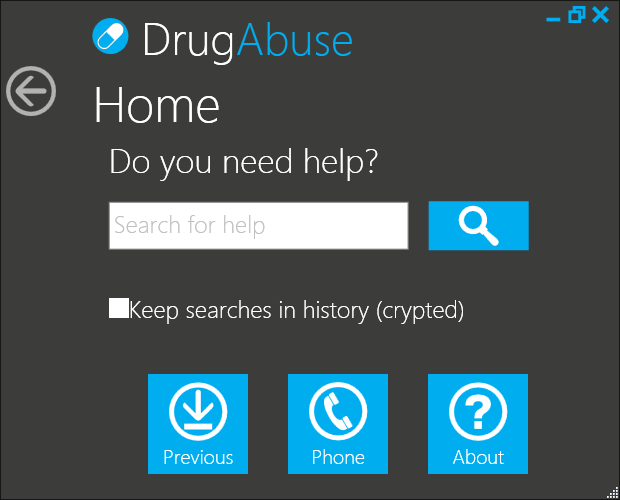
\includegraphics[width=0.35\textwidth]{images/desktop_screen_home.png}
\label{desktop_home}
~\\~\\

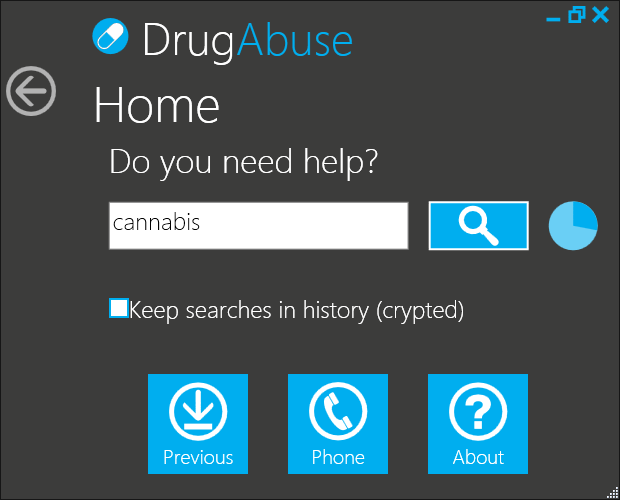
\includegraphics[width=0.35\textwidth]{images/desktop_screen_home_dl.png}
\label{desktop_dl}
~\\~\\

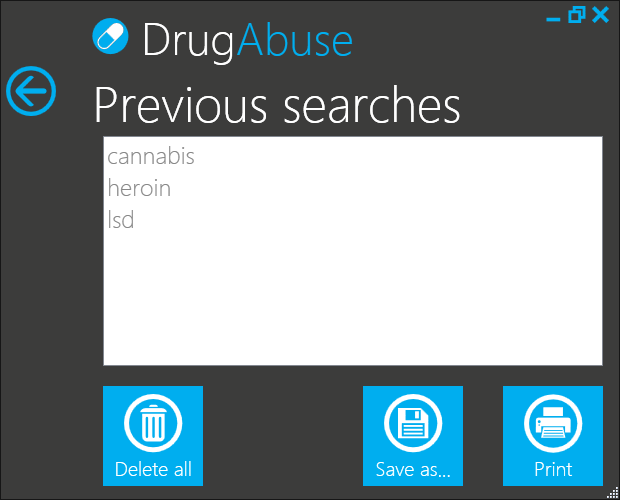
\includegraphics[width=0.35\textwidth]{images/desktop_screen_previous.png}
\label{desktop_previous}
~\\~\\

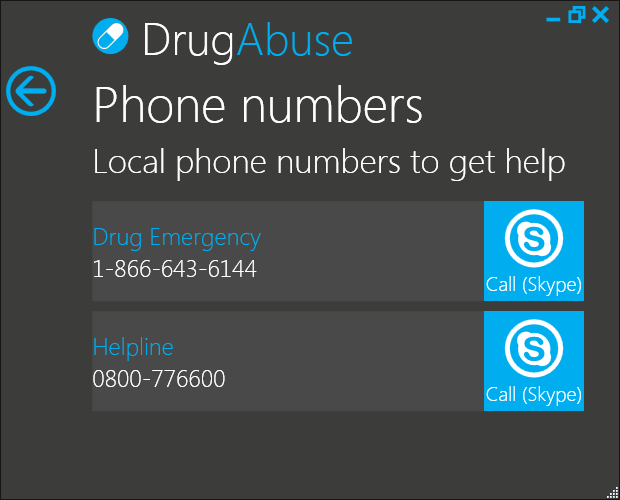
\includegraphics[width=0.35\textwidth]{images/desktop_screen_phone.png}
\label{desktop_phone}
~\\~\\

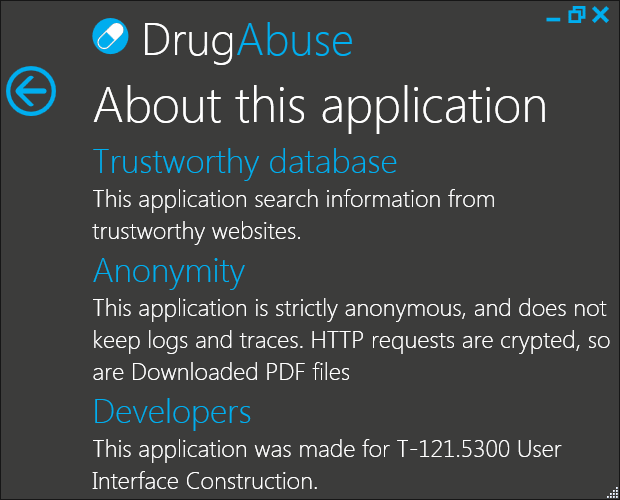
\includegraphics[width=0.35\textwidth]{images/desktop_screen_about.png}
\label{desktop_about}
\end{center}

%%%%%%% CLI %%%%%%%
\subsection{CLI screenshots}

\begin{center}
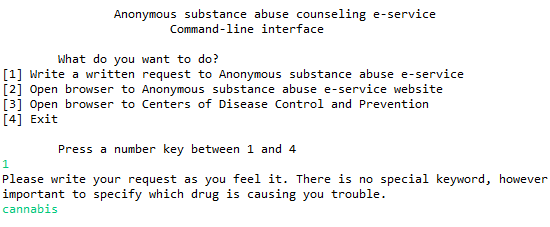
\includegraphics[width=0.5\textwidth]{images/cli_screen_1.png}
\label{cli_1}
~\\~\\

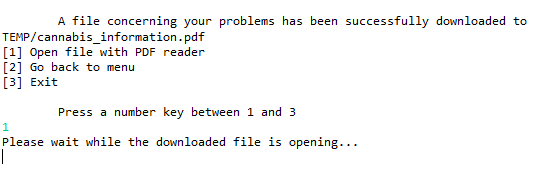
\includegraphics[width=0.5\textwidth]{images/cli_screen_2.png}
\label{cli_1}
\end{center}



%%%%%%%%%%%%%%%%%% BIBLIOGRAPHY %%%%%%%%%%%%%%%%%%

\begin{thebibliography}{9}

\bibitem{foobar2000}
  Bar, F. and Qux, B. 2000. \emph{how do you turn this on}.	% May actually use APA-style citing, as provided by Google Scholar for instance
\bibitem{windowsux} Microsoft Windows UX Design Principles. Available on the Web: http://msdn.microsoft.com/en-us/library/dd834141\%28v=MSDN.10\%29.aspx

%http://www.stephanemassey.com/metro-design-principles/
%http://en.wikipedia.org/wiki/Metro_(design_language)
\end{thebibliography}

\end{document}
